% Options for packages loaded elsewhere
\PassOptionsToPackage{unicode}{hyperref}
\PassOptionsToPackage{hyphens}{url}
\PassOptionsToPackage{dvipsnames,svgnames,x11names}{xcolor}
%
\documentclass[
  letterpaper,
  DIV=11,
  numbers=noendperiod]{scrartcl}

\usepackage{amsmath,amssymb}
\usepackage{iftex}
\ifPDFTeX
  \usepackage[T1]{fontenc}
  \usepackage[utf8]{inputenc}
  \usepackage{textcomp} % provide euro and other symbols
\else % if luatex or xetex
  \usepackage{unicode-math}
  \defaultfontfeatures{Scale=MatchLowercase}
  \defaultfontfeatures[\rmfamily]{Ligatures=TeX,Scale=1}
\fi
\usepackage{lmodern}
\ifPDFTeX\else  
    % xetex/luatex font selection
\fi
% Use upquote if available, for straight quotes in verbatim environments
\IfFileExists{upquote.sty}{\usepackage{upquote}}{}
\IfFileExists{microtype.sty}{% use microtype if available
  \usepackage[]{microtype}
  \UseMicrotypeSet[protrusion]{basicmath} % disable protrusion for tt fonts
}{}
\makeatletter
\@ifundefined{KOMAClassName}{% if non-KOMA class
  \IfFileExists{parskip.sty}{%
    \usepackage{parskip}
  }{% else
    \setlength{\parindent}{0pt}
    \setlength{\parskip}{6pt plus 2pt minus 1pt}}
}{% if KOMA class
  \KOMAoptions{parskip=half}}
\makeatother
\usepackage{xcolor}
\setlength{\emergencystretch}{3em} % prevent overfull lines
\setcounter{secnumdepth}{-\maxdimen} % remove section numbering
% Make \paragraph and \subparagraph free-standing
\ifx\paragraph\undefined\else
  \let\oldparagraph\paragraph
  \renewcommand{\paragraph}[1]{\oldparagraph{#1}\mbox{}}
\fi
\ifx\subparagraph\undefined\else
  \let\oldsubparagraph\subparagraph
  \renewcommand{\subparagraph}[1]{\oldsubparagraph{#1}\mbox{}}
\fi

\usepackage{color}
\usepackage{fancyvrb}
\newcommand{\VerbBar}{|}
\newcommand{\VERB}{\Verb[commandchars=\\\{\}]}
\DefineVerbatimEnvironment{Highlighting}{Verbatim}{commandchars=\\\{\}}
% Add ',fontsize=\small' for more characters per line
\usepackage{framed}
\definecolor{shadecolor}{RGB}{241,243,245}
\newenvironment{Shaded}{\begin{snugshade}}{\end{snugshade}}
\newcommand{\AlertTok}[1]{\textcolor[rgb]{0.68,0.00,0.00}{#1}}
\newcommand{\AnnotationTok}[1]{\textcolor[rgb]{0.37,0.37,0.37}{#1}}
\newcommand{\AttributeTok}[1]{\textcolor[rgb]{0.40,0.45,0.13}{#1}}
\newcommand{\BaseNTok}[1]{\textcolor[rgb]{0.68,0.00,0.00}{#1}}
\newcommand{\BuiltInTok}[1]{\textcolor[rgb]{0.00,0.23,0.31}{#1}}
\newcommand{\CharTok}[1]{\textcolor[rgb]{0.13,0.47,0.30}{#1}}
\newcommand{\CommentTok}[1]{\textcolor[rgb]{0.37,0.37,0.37}{#1}}
\newcommand{\CommentVarTok}[1]{\textcolor[rgb]{0.37,0.37,0.37}{\textit{#1}}}
\newcommand{\ConstantTok}[1]{\textcolor[rgb]{0.56,0.35,0.01}{#1}}
\newcommand{\ControlFlowTok}[1]{\textcolor[rgb]{0.00,0.23,0.31}{#1}}
\newcommand{\DataTypeTok}[1]{\textcolor[rgb]{0.68,0.00,0.00}{#1}}
\newcommand{\DecValTok}[1]{\textcolor[rgb]{0.68,0.00,0.00}{#1}}
\newcommand{\DocumentationTok}[1]{\textcolor[rgb]{0.37,0.37,0.37}{\textit{#1}}}
\newcommand{\ErrorTok}[1]{\textcolor[rgb]{0.68,0.00,0.00}{#1}}
\newcommand{\ExtensionTok}[1]{\textcolor[rgb]{0.00,0.23,0.31}{#1}}
\newcommand{\FloatTok}[1]{\textcolor[rgb]{0.68,0.00,0.00}{#1}}
\newcommand{\FunctionTok}[1]{\textcolor[rgb]{0.28,0.35,0.67}{#1}}
\newcommand{\ImportTok}[1]{\textcolor[rgb]{0.00,0.46,0.62}{#1}}
\newcommand{\InformationTok}[1]{\textcolor[rgb]{0.37,0.37,0.37}{#1}}
\newcommand{\KeywordTok}[1]{\textcolor[rgb]{0.00,0.23,0.31}{#1}}
\newcommand{\NormalTok}[1]{\textcolor[rgb]{0.00,0.23,0.31}{#1}}
\newcommand{\OperatorTok}[1]{\textcolor[rgb]{0.37,0.37,0.37}{#1}}
\newcommand{\OtherTok}[1]{\textcolor[rgb]{0.00,0.23,0.31}{#1}}
\newcommand{\PreprocessorTok}[1]{\textcolor[rgb]{0.68,0.00,0.00}{#1}}
\newcommand{\RegionMarkerTok}[1]{\textcolor[rgb]{0.00,0.23,0.31}{#1}}
\newcommand{\SpecialCharTok}[1]{\textcolor[rgb]{0.37,0.37,0.37}{#1}}
\newcommand{\SpecialStringTok}[1]{\textcolor[rgb]{0.13,0.47,0.30}{#1}}
\newcommand{\StringTok}[1]{\textcolor[rgb]{0.13,0.47,0.30}{#1}}
\newcommand{\VariableTok}[1]{\textcolor[rgb]{0.07,0.07,0.07}{#1}}
\newcommand{\VerbatimStringTok}[1]{\textcolor[rgb]{0.13,0.47,0.30}{#1}}
\newcommand{\WarningTok}[1]{\textcolor[rgb]{0.37,0.37,0.37}{\textit{#1}}}

\providecommand{\tightlist}{%
  \setlength{\itemsep}{0pt}\setlength{\parskip}{0pt}}\usepackage{longtable,booktabs,array}
\usepackage{calc} % for calculating minipage widths
% Correct order of tables after \paragraph or \subparagraph
\usepackage{etoolbox}
\makeatletter
\patchcmd\longtable{\par}{\if@noskipsec\mbox{}\fi\par}{}{}
\makeatother
% Allow footnotes in longtable head/foot
\IfFileExists{footnotehyper.sty}{\usepackage{footnotehyper}}{\usepackage{footnote}}
\makesavenoteenv{longtable}
\usepackage{graphicx}
\makeatletter
\def\maxwidth{\ifdim\Gin@nat@width>\linewidth\linewidth\else\Gin@nat@width\fi}
\def\maxheight{\ifdim\Gin@nat@height>\textheight\textheight\else\Gin@nat@height\fi}
\makeatother
% Scale images if necessary, so that they will not overflow the page
% margins by default, and it is still possible to overwrite the defaults
% using explicit options in \includegraphics[width, height, ...]{}
\setkeys{Gin}{width=\maxwidth,height=\maxheight,keepaspectratio}
% Set default figure placement to htbp
\makeatletter
\def\fps@figure{htbp}
\makeatother

\KOMAoption{captions}{tableheading}
\makeatletter
\@ifpackageloaded{caption}{}{\usepackage{caption}}
\AtBeginDocument{%
\ifdefined\contentsname
  \renewcommand*\contentsname{Table of contents}
\else
  \newcommand\contentsname{Table of contents}
\fi
\ifdefined\listfigurename
  \renewcommand*\listfigurename{List of Figures}
\else
  \newcommand\listfigurename{List of Figures}
\fi
\ifdefined\listtablename
  \renewcommand*\listtablename{List of Tables}
\else
  \newcommand\listtablename{List of Tables}
\fi
\ifdefined\figurename
  \renewcommand*\figurename{Figure}
\else
  \newcommand\figurename{Figure}
\fi
\ifdefined\tablename
  \renewcommand*\tablename{Table}
\else
  \newcommand\tablename{Table}
\fi
}
\@ifpackageloaded{float}{}{\usepackage{float}}
\floatstyle{ruled}
\@ifundefined{c@chapter}{\newfloat{codelisting}{h}{lop}}{\newfloat{codelisting}{h}{lop}[chapter]}
\floatname{codelisting}{Listing}
\newcommand*\listoflistings{\listof{codelisting}{List of Listings}}
\makeatother
\makeatletter
\makeatother
\makeatletter
\@ifpackageloaded{caption}{}{\usepackage{caption}}
\@ifpackageloaded{subcaption}{}{\usepackage{subcaption}}
\makeatother
\ifLuaTeX
  \usepackage{selnolig}  % disable illegal ligatures
\fi
\usepackage{bookmark}

\IfFileExists{xurl.sty}{\usepackage{xurl}}{} % add URL line breaks if available
\urlstyle{same} % disable monospaced font for URLs
\hypersetup{
  pdftitle={Maryland Hospital Emergency Department Wait Times},
  colorlinks=true,
  linkcolor={blue},
  filecolor={Maroon},
  citecolor={Blue},
  urlcolor={Blue},
  pdfcreator={LaTeX via pandoc}}

\title{Maryland Hospital Emergency Department Wait Times}
\author{}
\date{}

\begin{document}
\maketitle

In June, the Maryland Hospitals Association established EDDIE, the
Emergency Department Dramatic Improvements Effort, to address hospital
wait times in the state. By having each hospital set objectives for
lowering emergency department wait times and discharges, EDDIE aims to
put Maryland hospitals back on target with the rest of the country. Now,
the state has one of the highest average wait times in the country.
EDDIE has been collecting monthly data on each Maryland hospital's
average wait times, and I have that data from July 2023 through January
2024, provided by a request to the Maryland Hospital Association.

The data provided by the MHA is fairly large and consists of numerous
variables.

ED1 refers to emergency department ``arrival to inpatient a admission
time'' and OP refers outpatients who are discharged into the community
for ``outpatient ED arrival to discharge time'' according to Damiara
Smith, a quality fellow for the MHA cost review commission.

For this project, I have chosen to analyze the aggregated psych and
non-psych sheet columns to measure hospital patient arrival to emergency
department admission on a general basis for all patients, as opposed to
psych or non-psych.

Research Questions:

\begin{enumerate}
\def\labelenumi{\arabic{enumi}.}
\tightlist
\item
  What are the average wait times for each hospital across the state in
  January in hours? As of January, what is month over month wait time
  for the hospitals with the longst and shortest wait times?
\item
  What hospitals in Maryland are seeing the most and least improvement
  in wait times? 1a. Which 5 hospitals had the lowest percent change
  since base month? 1b. How many hospitals have had increasing wait
  times from their base month to January? Which 5 have had the biggest
  increases?
\item
  How does Maryland's average ED wait time compare to the rest of the
  country?
\item
  Are there any patterns between urban and rural hospitals? What factors
  affect wait times in each of these areas?
\item
  What hospital has seen the most improvement (and least) in its
  hospital wait times?
\end{enumerate}

\#Data Notebook

Q1: What hospitals in Maryland are seeing the most and least
improvement? Which 5 hospitals had the lowest percent change since
August?

\begin{Shaded}
\begin{Highlighting}[]
\CommentTok{\#A {-} Load libraries}

\FunctionTok{library}\NormalTok{(tidyverse)}
\end{Highlighting}
\end{Shaded}

\begin{verbatim}
-- Attaching core tidyverse packages ------------------------ tidyverse 2.0.0 --
v dplyr     1.1.4     v readr     2.1.5
v forcats   1.0.0     v stringr   1.5.1
v ggplot2   3.4.4     v tibble    3.2.1
v lubridate 1.9.3     v tidyr     1.3.1
v purrr     1.0.2     
-- Conflicts ------------------------------------------ tidyverse_conflicts() --
x dplyr::filter() masks stats::filter()
x dplyr::lag()    masks stats::lag()
i Use the conflicted package (<http://conflicted.r-lib.org/>) to force all conflicts to become errors
\end{verbatim}

\begin{Shaded}
\begin{Highlighting}[]
\FunctionTok{library}\NormalTok{(rio)}
\FunctionTok{library}\NormalTok{(janitor)}
\end{Highlighting}
\end{Shaded}

\begin{verbatim}

Attaching package: 'janitor'

The following objects are masked from 'package:stats':

    chisq.test, fisher.test
\end{verbatim}

\begin{Shaded}
\begin{Highlighting}[]
\FunctionTok{library}\NormalTok{(readr)}

\FunctionTok{install\_formats}\NormalTok{()}
\FunctionTok{library}\NormalTok{(conflicted)}
\FunctionTok{conflict\_prefer}\NormalTok{(}\StringTok{"filter"}\NormalTok{, }\StringTok{"dplyr"}\NormalTok{)}
\end{Highlighting}
\end{Shaded}

\begin{verbatim}
[conflicted] Will prefer dplyr::filter over any other package.
\end{verbatim}

\begin{Shaded}
\begin{Highlighting}[]
\FunctionTok{conflict\_prefer}\NormalTok{(}\StringTok{"lag"}\NormalTok{, }\StringTok{"dplyr"}\NormalTok{)}
\end{Highlighting}
\end{Shaded}

\begin{verbatim}
[conflicted] Will prefer dplyr::lag over any other package.
\end{verbatim}

\begin{Shaded}
\begin{Highlighting}[]
\FunctionTok{library}\NormalTok{(dplyr)}
\FunctionTok{library}\NormalTok{(stringr)}
\end{Highlighting}
\end{Shaded}

\begin{Shaded}
\begin{Highlighting}[]
\CommentTok{\#B {-} Import the data}

\NormalTok{ED1a }\OtherTok{\textless{}{-}}\NormalTok{ rio}\SpecialCharTok{::}\FunctionTok{import}\NormalTok{(}\StringTok{"EDDIE January FINAL.xlsx"}\NormalTok{, }\AttributeTok{sheet=}\StringTok{"ED1a"}\NormalTok{)}
\end{Highlighting}
\end{Shaded}

\begin{verbatim}
New names:
* `` -> `...21`
\end{verbatim}

\begin{Shaded}
\begin{Highlighting}[]
\NormalTok{ED1a }\OtherTok{\textless{}{-}} \FunctionTok{clean\_names}\NormalTok{(ED1a)}
\end{Highlighting}
\end{Shaded}

Q1: What are the average wait times for each hospital across the state
in January in hours? As of January, what is month over month wait time
for the hospitals with the longst and shortest wait times?

\begin{Shaded}
\begin{Highlighting}[]
\CommentTok{\#Heat map of hospitals}
\NormalTok{january\_ed }\OtherTok{\textless{}{-}}\NormalTok{ ED1a }\SpecialCharTok{\%\textgreater{}\%} 
  \FunctionTok{select}\NormalTok{(abbreviated\_name, january\_median) }\SpecialCharTok{\%\textgreater{}\%} 
  \FunctionTok{mutate}\NormalTok{(}\AttributeTok{address =}\NormalTok{ abbreviated\_name) }\SpecialCharTok{\%\textgreater{}\%} 
  \FunctionTok{head}\NormalTok{(}\DecValTok{41}\NormalTok{)}

\NormalTok{january\_ed}\SpecialCharTok{$}\NormalTok{address}\OtherTok{\textless{}{-}} \FunctionTok{gsub}\NormalTok{(}\StringTok{"Frederick"}\NormalTok{, }\StringTok{"400 W 7th St, Frederick, MD 21701"}\NormalTok{, january\_ed}\SpecialCharTok{$}\NormalTok{address)}
\NormalTok{january\_ed}\SpecialCharTok{$}\NormalTok{address}\OtherTok{\textless{}{-}} \FunctionTok{gsub}\NormalTok{(}\StringTok{"Carroll"}\NormalTok{, }\StringTok{"200 Memorial Ave, Westminster, MD 21157"}\NormalTok{, january\_ed}\SpecialCharTok{$}\NormalTok{address)}
\NormalTok{january\_ed}\SpecialCharTok{$}\NormalTok{address}\OtherTok{\textless{}{-}} \FunctionTok{gsub}\NormalTok{(}\StringTok{"Atlantic General"}\NormalTok{, }\StringTok{"9733 Healthway Dr, Berlin, MD 21811"}\NormalTok{, january\_ed}\SpecialCharTok{$}\NormalTok{address)}
\NormalTok{january\_ed}\SpecialCharTok{$}\NormalTok{address}\OtherTok{\textless{}{-}} \FunctionTok{gsub}\NormalTok{(}\StringTok{"Garrett"}\NormalTok{, }\StringTok{"251 N 4th St, Oakland, MD 21550"}\NormalTok{, january\_ed}\SpecialCharTok{$}\NormalTok{address)}
\NormalTok{january\_ed}\SpecialCharTok{$}\NormalTok{address}\OtherTok{\textless{}{-}} \FunctionTok{gsub}\NormalTok{(}\StringTok{"MedStar St. Mary\textquotesingle{}s"}\NormalTok{, }\StringTok{"25500 Point Lookout Rd, Leonardtown, MD 20650"}\NormalTok{, january\_ed}\SpecialCharTok{$}\NormalTok{address)}
\NormalTok{january\_ed}\SpecialCharTok{$}\NormalTok{address}\OtherTok{\textless{}{-}} \FunctionTok{gsub}\NormalTok{(}\StringTok{"Calvert"}\NormalTok{, }\StringTok{"100 Hospital Rd, Prince Frederick, MD 20678"}\NormalTok{, january\_ed}\SpecialCharTok{$}\NormalTok{address)}
\NormalTok{january\_ed}\SpecialCharTok{$}\NormalTok{address}\OtherTok{\textless{}{-}} \FunctionTok{gsub}\NormalTok{(}\StringTok{"Meritus"}\NormalTok{, }\StringTok{"11116 Medical Campus Rd, Hagerstown, MD 21742"}\NormalTok{, january\_ed}\SpecialCharTok{$}\NormalTok{address)}
\NormalTok{january\_ed}\SpecialCharTok{$}\NormalTok{address}\OtherTok{\textless{}{-}} \FunctionTok{gsub}\NormalTok{(}\StringTok{"MedStar Union Memorial"}\NormalTok{, }\StringTok{"201 E University Pkwy, Baltimore, MD 21218"}\NormalTok{, january\_ed}\SpecialCharTok{$}\NormalTok{address)}
\NormalTok{january\_ed}\SpecialCharTok{$}\NormalTok{address}\OtherTok{\textless{}{-}} \FunctionTok{gsub}\NormalTok{(}\StringTok{"ChristianaCare, Union"}\NormalTok{, }\StringTok{"106 Bow St, Elkton, MD 21921"}\NormalTok{, january\_ed}\SpecialCharTok{$}\NormalTok{address)}
\NormalTok{january\_ed}\SpecialCharTok{$}\NormalTok{address}\OtherTok{\textless{}{-}} \FunctionTok{gsub}\NormalTok{(}\StringTok{"TidalHealth Peninsula"}\NormalTok{, }\StringTok{"100 E Carroll St, Salisbury, MD 21801"}\NormalTok{, january\_ed}\SpecialCharTok{$}\NormalTok{address)}
\NormalTok{january\_ed}\SpecialCharTok{$}\NormalTok{address}\OtherTok{\textless{}{-}} \FunctionTok{gsub}\NormalTok{(}\StringTok{"GBMC"}\NormalTok{, }\StringTok{"19801 Observation Dr, Germantown, MD 20876"}\NormalTok{, january\_ed}\SpecialCharTok{$}\NormalTok{address)}
\NormalTok{january\_ed}\SpecialCharTok{$}\NormalTok{address}\OtherTok{\textless{}{-}} \FunctionTok{gsub}\NormalTok{(}\StringTok{"Holy Cross Germantown"}\NormalTok{, }\StringTok{"251 N 4th St, Oakland, MD 21550"}\NormalTok{, january\_ed}\SpecialCharTok{$}\NormalTok{address)}
\NormalTok{january\_ed}\SpecialCharTok{$}\NormalTok{address}\OtherTok{\textless{}{-}} \FunctionTok{gsub}\NormalTok{(}\StringTok{"HARFORD MEMORIAL"}\NormalTok{, }\StringTok{" 501 S Union Ave, Havre De Grace, MD 21078"}\NormalTok{, january\_ed}\SpecialCharTok{$}\NormalTok{address)}
\NormalTok{january\_ed}\SpecialCharTok{$}\NormalTok{address}\OtherTok{\textless{}{-}} \FunctionTok{gsub}\NormalTok{(}\StringTok{"Ft. Washington"}\NormalTok{, }\StringTok{"11711 Livingston Rd, Fort Washington, MD 20744"}\NormalTok{, january\_ed}\SpecialCharTok{$}\NormalTok{address)}
\NormalTok{january\_ed}\SpecialCharTok{$}\NormalTok{address}\OtherTok{\textless{}{-}} \FunctionTok{gsub}\NormalTok{(}\StringTok{"Shady Grove"}\NormalTok{, }\StringTok{"9901 Medical Center Dr, Rockville, MD 20850"}\NormalTok{, january\_ed}\SpecialCharTok{$}\NormalTok{address)}
\NormalTok{january\_ed}\SpecialCharTok{$}\NormalTok{address}\OtherTok{\textless{}{-}} \FunctionTok{gsub}\NormalTok{(}\StringTok{"Mercy"}\NormalTok{, }\StringTok{"301 St Paul St, Baltimore, MD 21202"}\NormalTok{, january\_ed}\SpecialCharTok{$}\NormalTok{address)}
\NormalTok{january\_ed}\SpecialCharTok{$}\NormalTok{address}\OtherTok{\textless{}{-}} \FunctionTok{gsub}\NormalTok{(}\StringTok{"UPMC Western MD"}\NormalTok{, }\StringTok{"12500 Willowbrook Rd, Cumberland, MD 21502"}\NormalTok{, january\_ed}\SpecialCharTok{$}\NormalTok{address)}
\NormalTok{january\_ed}\SpecialCharTok{$}\NormalTok{address}\OtherTok{\textless{}{-}} \FunctionTok{gsub}\NormalTok{(}\StringTok{"Suburban"}\NormalTok{, }\StringTok{"8600 Old Georgetown Rd, Bethesda, MD 20814"}\NormalTok{, january\_ed}\SpecialCharTok{$}\NormalTok{address)}
\NormalTok{january\_ed}\SpecialCharTok{$}\NormalTok{address}\OtherTok{\textless{}{-}} \FunctionTok{gsub}\NormalTok{(}\StringTok{"MedStar Montgomery"}\NormalTok{, }\StringTok{"18101 Prince Philip Dr, Olney, MD 20832"}\NormalTok{, january\_ed}\SpecialCharTok{$}\NormalTok{address)}
\NormalTok{january\_ed}\SpecialCharTok{$}\NormalTok{address}\OtherTok{\textless{}{-}} \FunctionTok{gsub}\NormalTok{(}\StringTok{"CHARLES REGIONAL"}\NormalTok{, }\StringTok{"5 Garrett Ave, La Plata, MD 20646"}\NormalTok{, january\_ed}\SpecialCharTok{$}\NormalTok{address)}
\NormalTok{january\_ed}\SpecialCharTok{$}\NormalTok{address}\OtherTok{\textless{}{-}} \FunctionTok{gsub}\NormalTok{(}\StringTok{"MedStar Franklin Square"}\NormalTok{, }\StringTok{"9000 Franklin Square Dr, Baltimore, MD 21237"}\NormalTok{, january\_ed}\SpecialCharTok{$}\NormalTok{address)}
\NormalTok{january\_ed}\SpecialCharTok{$}\NormalTok{address}\OtherTok{\textless{}{-}} \FunctionTok{gsub}\NormalTok{(}\StringTok{"MedStar Harbor"}\NormalTok{, }\StringTok{"3001 S Hanover St, Baltimore, MD 21225"}\NormalTok{, january\_ed}\SpecialCharTok{$}\NormalTok{address)}
\NormalTok{january\_ed}\SpecialCharTok{$}\NormalTok{address}\OtherTok{\textless{}{-}} \FunctionTok{gsub}\NormalTok{(}\StringTok{"Holy Cross"}\NormalTok{, }\StringTok{"1500 Forest Glen Rd, Silver Spring, MD 20910"}\NormalTok{, january\_ed}\SpecialCharTok{$}\NormalTok{address)}
\NormalTok{january\_ed}\SpecialCharTok{$}\NormalTok{address}\OtherTok{\textless{}{-}} \FunctionTok{gsub}\NormalTok{(}\StringTok{"Doctors"}\NormalTok{, }\StringTok{"2121 Medical Park Dr, Silver Spring, MD 20902"}\NormalTok{, january\_ed}\SpecialCharTok{$}\NormalTok{address)}
\NormalTok{january\_ed}\SpecialCharTok{$}\NormalTok{address}\OtherTok{\textless{}{-}} \FunctionTok{gsub}\NormalTok{(}\StringTok{"AAMC"}\NormalTok{, }\StringTok{"2001 Medical Pkwy, Annapolis, MD 21401"}\NormalTok{, january\_ed}\SpecialCharTok{$}\NormalTok{address)}
\NormalTok{january\_ed}\SpecialCharTok{$}\NormalTok{address}\OtherTok{\textless{}{-}} \FunctionTok{gsub}\NormalTok{(}\StringTok{"MedStar Good Samaritan"}\NormalTok{, }\StringTok{"5601 Loch Raven Blvd, Baltimore, MD 21239"}\NormalTok{, january\_ed}\SpecialCharTok{$}\NormalTok{address)}
\NormalTok{january\_ed}\SpecialCharTok{$}\NormalTok{address}\OtherTok{\textless{}{-}} \FunctionTok{gsub}\NormalTok{(}\StringTok{"MedStar Southern Maryland"}\NormalTok{, }\StringTok{"7503 Surratts Rd, Clinton, MD 20735"}\NormalTok{, january\_ed}\SpecialCharTok{$}\NormalTok{address)}
\NormalTok{january\_ed}\SpecialCharTok{$}\NormalTok{address}\OtherTok{\textless{}{-}} \FunctionTok{gsub}\NormalTok{(}\StringTok{"Ascension Saint Agnes"}\NormalTok{, }\StringTok{"900 S Caton Ave, Baltimore, MD 21229"}\NormalTok{, january\_ed}\SpecialCharTok{$}\NormalTok{address)}
\NormalTok{january\_ed}\SpecialCharTok{$}\NormalTok{address}\OtherTok{\textless{}{-}} \FunctionTok{gsub}\NormalTok{(}\StringTok{"UM ST. JOSEPH"}\NormalTok{, }\StringTok{"7601 Osler Drive Towson, MD 21204"}\NormalTok{, january\_ed}\SpecialCharTok{$}\NormalTok{address)}
\NormalTok{january\_ed}\SpecialCharTok{$}\NormalTok{address}\OtherTok{\textless{}{-}} \FunctionTok{gsub}\NormalTok{(}\StringTok{"UMMC Downtown"}\NormalTok{, }\StringTok{"22 S Greene St, Baltimore, MD 21201"}\NormalTok{, january\_ed}\SpecialCharTok{$}\NormalTok{address)}
\NormalTok{january\_ed}\SpecialCharTok{$}\NormalTok{address}\OtherTok{\textless{}{-}} \FunctionTok{gsub}\NormalTok{(}\StringTok{"Northwest"}\NormalTok{, }\StringTok{"5401 Old Court Rd, Randallstown, MD 21133"}\NormalTok{, january\_ed}\SpecialCharTok{$}\NormalTok{address)}
\NormalTok{january\_ed}\SpecialCharTok{$}\NormalTok{address}\OtherTok{\textless{}{-}} \FunctionTok{gsub}\NormalTok{(}\StringTok{"UMMC MIDTOWN"}\NormalTok{, }\StringTok{"800 Linden Ave 10th Floor, Baltimore, MD 21201"}\NormalTok{, january\_ed}\SpecialCharTok{$}\NormalTok{address)}
\NormalTok{january\_ed}\SpecialCharTok{$}\NormalTok{address}\OtherTok{\textless{}{-}} \FunctionTok{gsub}\NormalTok{(}\StringTok{"Johns Hopkins"}\NormalTok{, }\StringTok{"1800 Orleans St, Baltimore, MD 21287"}\NormalTok{, january\_ed}\SpecialCharTok{$}\NormalTok{address)}
\NormalTok{january\_ed}\SpecialCharTok{$}\NormalTok{address}\OtherTok{\textless{}{-}} \FunctionTok{gsub}\NormalTok{(}\StringTok{"UM BWMC"}\NormalTok{, }\StringTok{"301 Hospital Dr, Glen Burnie, MD 21061"}\NormalTok{, january\_ed}\SpecialCharTok{$}\NormalTok{address)}
\NormalTok{january\_ed}\SpecialCharTok{$}\NormalTok{address}\OtherTok{\textless{}{-}} \FunctionTok{gsub}\NormalTok{(}\StringTok{"Howard"}\NormalTok{, }\StringTok{"2041 Georgia Ave NW, Washington, DC 20060"}\NormalTok{, january\_ed}\SpecialCharTok{$}\NormalTok{address)}
\NormalTok{january\_ed}\SpecialCharTok{$}\NormalTok{address}\OtherTok{\textless{}{-}} \FunctionTok{gsub}\NormalTok{(}\StringTok{"Sinai"}\NormalTok{, }\StringTok{"2401 W Belvedere Ave, Baltimore, MD 21215"}\NormalTok{, january\_ed}\SpecialCharTok{$}\NormalTok{address)}
\NormalTok{january\_ed}\SpecialCharTok{$}\NormalTok{address}\OtherTok{\textless{}{-}} \FunctionTok{gsub}\NormalTok{(}\StringTok{"UPPER CHESAPEAKE"}\NormalTok{, }\StringTok{"500 Upper Chesapeake Dr, Bel Air, MD 21014"}\NormalTok{, january\_ed}\SpecialCharTok{$}\NormalTok{address)}
\NormalTok{january\_ed}\SpecialCharTok{$}\NormalTok{address}\OtherTok{\textless{}{-}} \FunctionTok{gsub}\NormalTok{(}\StringTok{"UM CAPITAL REGION"}\NormalTok{, }\StringTok{"901 Harry S Truman Dr, Largo, MD 20774"}\NormalTok{, january\_ed}\SpecialCharTok{$}\NormalTok{address)}
\NormalTok{january\_ed}\SpecialCharTok{$}\NormalTok{address}\OtherTok{\textless{}{-}} \FunctionTok{gsub}\NormalTok{(}\StringTok{"White Oak"}\NormalTok{, }\StringTok{"11890 Healing Wy, Silver Spring, MD 20904"}\NormalTok{, january\_ed}\SpecialCharTok{$}\NormalTok{address)}
\NormalTok{january\_ed}\SpecialCharTok{$}\NormalTok{address}\OtherTok{\textless{}{-}} \FunctionTok{gsub}\NormalTok{(}\StringTok{"JH Bayview"}\NormalTok{, }\StringTok{"4940 Eastern Ave, Baltimore, MD 21224"}\NormalTok{, january\_ed}\SpecialCharTok{$}\NormalTok{address)}
\NormalTok{january\_ed}\SpecialCharTok{$}\NormalTok{address}\OtherTok{\textless{}{-}} \FunctionTok{gsub}\NormalTok{(}\StringTok{"UM SHORE EASTON"}\NormalTok{, }\StringTok{"219 S Washington St, Easton, MD 21601"}\NormalTok{, january\_ed}\SpecialCharTok{$}\NormalTok{address)}

\CommentTok{\#Some of the addresses over rode themsleves (for example in TidalHealth Peninsula hospital, "Carrol" in Caroll Street was overrode by Carroll hospital\textquotesingle{}s address. I fixed this in the csv file before uploading to Data Wrapper)}
\end{Highlighting}
\end{Shaded}

DO NOT RUN \#install.packages(``ggmap'') library(ggmap)
register\_google(key = ``XXXXX'')

january\_ed \textless- january\_ed \%\textgreater\% mutate(location =
geocode(address))

Map from data wrapper: https://app.datawrapper.de/map/BTfas/publish

\begin{Shaded}
\begin{Highlighting}[]
\NormalTok{january\_ed}\SpecialCharTok{$}\NormalTok{address\_back }\OtherTok{\textless{}{-}}\NormalTok{ january\_ed}\SpecialCharTok{$}\NormalTok{address}
\NormalTok{january\_ed}\OtherTok{\textless{}{-}} \FunctionTok{separate}\NormalTok{(january\_ed, }\AttributeTok{col =}\NormalTok{ address\_back, }\AttributeTok{into =} \FunctionTok{c}\NormalTok{(}\StringTok{"street"}\NormalTok{, }\StringTok{"city"}\NormalTok{, }\StringTok{"zip"}\NormalTok{), }\AttributeTok{sep =} \StringTok{","}\NormalTok{, }\AttributeTok{extra =} \StringTok{"merge"}\NormalTok{, }\AttributeTok{fill =} \StringTok{"right"}\NormalTok{) }\SpecialCharTok{\%\textgreater{}\%} 
  \FunctionTok{mutate}\NormalTok{(}\AttributeTok{city=}\FunctionTok{str\_squish}\NormalTok{(city))}
  
\NormalTok{january\_ed }\OtherTok{\textless{}{-}} \FunctionTok{separate}\NormalTok{(january\_ed, }\AttributeTok{col =}\NormalTok{ zip, }\AttributeTok{into =} \FunctionTok{c}\NormalTok{(}\StringTok{"state"}\NormalTok{, }\StringTok{"zip"}\NormalTok{), }\AttributeTok{sep =} \StringTok{"MD "}\NormalTok{)}
\end{Highlighting}
\end{Shaded}

\begin{verbatim}
Warning: Expected 2 pieces. Missing pieces filled with `NA` in 1 rows [35].
\end{verbatim}

\begin{Shaded}
\begin{Highlighting}[]
\NormalTok{january\_ed }\OtherTok{\textless{}{-}}\NormalTok{january\_ed }\SpecialCharTok{\%\textgreater{}\%} 
  \FunctionTok{mutate}\NormalTok{(}\AttributeTok{state=} \StringTok{"MD"}\NormalTok{)}

\NormalTok{january\_ed }\OtherTok{\textless{}{-}}\NormalTok{january\_ed }\SpecialCharTok{\%\textgreater{}\%} 
  \FunctionTok{mutate}\NormalTok{(}\AttributeTok{median\_hour =} \FunctionTok{round}\NormalTok{(january\_median}\SpecialCharTok{/}\DecValTok{60}\NormalTok{, }\DecValTok{2}\NormalTok{))}
  
\NormalTok{january\_ed }\OtherTok{\textless{}{-}} \FunctionTok{clean\_names}\NormalTok{(january\_ed)}

\FunctionTok{write.csv}\NormalTok{(january\_ed, }\StringTok{"january\_ed.csv"}\NormalTok{)}
\end{Highlighting}
\end{Shaded}

\begin{Shaded}
\begin{Highlighting}[]
\CommentTok{\#Hospital with longest wait time in January}

\NormalTok{longest }\OtherTok{\textless{}{-}}\NormalTok{ ED1a }\SpecialCharTok{\%\textgreater{}\%} 
  \FunctionTok{select}\NormalTok{(abbreviated\_name, january\_median) }\SpecialCharTok{\%\textgreater{}\%} 
  \FunctionTok{arrange}\NormalTok{(}\FunctionTok{desc}\NormalTok{(january\_median))}


\CommentTok{\#In January, University of Maryland Shore Eastern in Easton, Md. (Talbot County) had the longest wait time at 1770.5 minutes, or 29.5 hours.}


\NormalTok{longest\_graph }\OtherTok{\textless{}{-}}\NormalTok{ rio}\SpecialCharTok{::}\FunctionTok{import}\NormalTok{(}\StringTok{"EDDIE January FINAL.xlsx"}\NormalTok{, }\AttributeTok{sheet=}\StringTok{"UMES"}\NormalTok{)}

\NormalTok{longest\_graph }\OtherTok{\textless{}{-}} \FunctionTok{clean\_names}\NormalTok{(longest\_graph)}

\NormalTok{longest\_graph }\OtherTok{\textless{}{-}}\NormalTok{ longest\_graph }\SpecialCharTok{\%\textgreater{}\%} 
  \FunctionTok{mutate}\NormalTok{(}\AttributeTok{month\_order=}\NormalTok{month) }


\NormalTok{longest\_graph }\OtherTok{\textless{}{-}}\NormalTok{ longest\_graph }\SpecialCharTok{\%\textgreater{}\%}
  \FunctionTok{mutate}\NormalTok{(}\AttributeTok{month\_order =} \FunctionTok{case\_when}\NormalTok{(}
\NormalTok{     month }\SpecialCharTok{==} \StringTok{"June"} \SpecialCharTok{\textasciitilde{}} \StringTok{"1"}\NormalTok{,}
\NormalTok{    month }\SpecialCharTok{==} \StringTok{"July"} \SpecialCharTok{\textasciitilde{}} \StringTok{"2"}\NormalTok{,}
\NormalTok{     month }\SpecialCharTok{==} \StringTok{"August"} \SpecialCharTok{\textasciitilde{}} \StringTok{"3"}\NormalTok{,}
\NormalTok{     month }\SpecialCharTok{==} \StringTok{"September"} \SpecialCharTok{\textasciitilde{}} \StringTok{"4"}\NormalTok{,}
\NormalTok{    month }\SpecialCharTok{==} \StringTok{"October"} \SpecialCharTok{\textasciitilde{}} \StringTok{"5"}\NormalTok{,}
\NormalTok{     month }\SpecialCharTok{==} \StringTok{"November"} \SpecialCharTok{\textasciitilde{}} \StringTok{"6"}\NormalTok{,}
\NormalTok{     month }\SpecialCharTok{==} \StringTok{"December"} \SpecialCharTok{\textasciitilde{}} \StringTok{"7"}\NormalTok{,}
\NormalTok{     month }\SpecialCharTok{==} \StringTok{"January"} \SpecialCharTok{\textasciitilde{}} \StringTok{"8"}
\NormalTok{   ))}

\NormalTok{longest\_graph }\OtherTok{\textless{}{-}}\NormalTok{ longest\_graph }\SpecialCharTok{\%\textgreater{}\%} 
  \FunctionTok{mutate}\NormalTok{(}\AttributeTok{median\_hour =} \FunctionTok{round}\NormalTok{(median}\SpecialCharTok{/}\DecValTok{60}\NormalTok{,}\DecValTok{2}\NormalTok{))}

\NormalTok{longest\_graph}\SpecialCharTok{$}\NormalTok{month }\OtherTok{\textless{}{-}} \FunctionTok{factor}\NormalTok{(longest\_graph}\SpecialCharTok{$}\NormalTok{month, }\AttributeTok{levels =}  \FunctionTok{c}\NormalTok{(}\StringTok{"June"}\NormalTok{, }\StringTok{"July"}\NormalTok{, }\StringTok{"August"}\NormalTok{, }\StringTok{"September"}\NormalTok{, }\StringTok{"October"}\NormalTok{, }\StringTok{"November"}\NormalTok{, }\StringTok{"December"}\NormalTok{, }\StringTok{"January"}\NormalTok{))}

\NormalTok{longest\_graph }\SpecialCharTok{\%\textgreater{}\%} 
  \FunctionTok{ggplot}\NormalTok{(}\FunctionTok{aes}\NormalTok{(}\AttributeTok{x=}\NormalTok{month, }\AttributeTok{y=}\NormalTok{median\_hour, }\AttributeTok{weight=}\NormalTok{median\_hour, }\AttributeTok{fill=}\NormalTok{month)) }\SpecialCharTok{+}
  \FunctionTok{geom\_col}\NormalTok{()}\SpecialCharTok{+}
  \FunctionTok{geom\_text}\NormalTok{(}\FunctionTok{aes}\NormalTok{(}\AttributeTok{label=}\NormalTok{median\_hour), }\AttributeTok{vjust =} \SpecialCharTok{{-}}\DecValTok{1}\NormalTok{, }\AttributeTok{size =} \FloatTok{2.5}\NormalTok{) }\SpecialCharTok{+}
  \FunctionTok{labs}\NormalTok{(}
    \AttributeTok{title=}\StringTok{"Median Time (in hours) by Month for UM Shore Eastern"}\NormalTok{,}
    \AttributeTok{x =} \StringTok{"Month"}\NormalTok{,}
    \AttributeTok{y =} \StringTok{"Median time in hours"}\NormalTok{,}
    \AttributeTok{caption =} \StringTok{"UM Eastern Shore\textquotesingle{}s hospital, based in Easton, Md., had the longest ER waittime in the state in January. }
\StringTok{    This shows median emergency department wait times for eight months at the hospital.}
\StringTok{    Source: Maryland Hospital Association Cost Review Commisssion"}\NormalTok{)}
\end{Highlighting}
\end{Shaded}

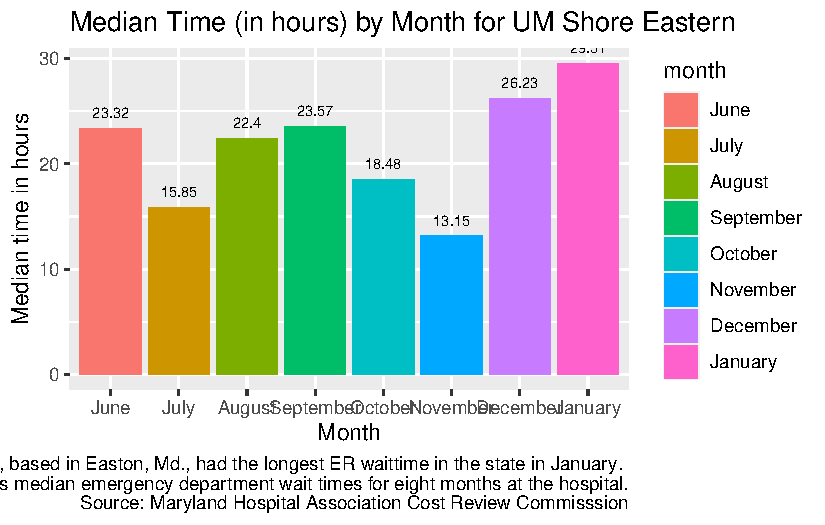
\includegraphics{Condon_MD_HOSPITAL_DATA_FINAL_files/figure-pdf/unnamed-chunk-5-1.pdf}

\begin{Shaded}
\begin{Highlighting}[]
\CommentTok{\#Hospital with shortest wait time in January}

\NormalTok{shortest }\OtherTok{\textless{}{-}}\NormalTok{ ED1a }\SpecialCharTok{\%\textgreater{}\%} 
  \FunctionTok{select}\NormalTok{(abbreviated\_name, january\_median) }\SpecialCharTok{\%\textgreater{}\%} 
  \FunctionTok{arrange}\NormalTok{(january\_median)}

\CommentTok{\#In January, Atlantic General, located in Berlin, Md (Worcester County) had the  shortest wait time at 193 minutes, or about 3.2 hours.}

\NormalTok{shortest\_graph }\OtherTok{\textless{}{-}}\NormalTok{ rio}\SpecialCharTok{::}\FunctionTok{import}\NormalTok{(}\StringTok{"EDDIE January FINAL.xlsx"}\NormalTok{, }\AttributeTok{sheet=}\StringTok{"AG"}\NormalTok{)}

\NormalTok{shortest\_graph }\OtherTok{\textless{}{-}} \FunctionTok{clean\_names}\NormalTok{(shortest\_graph)}

\NormalTok{shortest\_graph }\OtherTok{\textless{}{-}}\NormalTok{ shortest\_graph }\SpecialCharTok{\%\textgreater{}\%} 
  \FunctionTok{mutate}\NormalTok{(}\AttributeTok{month\_order=}\NormalTok{month) }

\NormalTok{shortest\_graph}\SpecialCharTok{$}\NormalTok{month\_order }\OtherTok{\textless{}{-}} \FunctionTok{gsub}\NormalTok{(}\StringTok{"June"}\NormalTok{, }\StringTok{"1"}\NormalTok{, shortest\_graph}\SpecialCharTok{$}\NormalTok{month\_order)}
\NormalTok{shortest\_graph}\SpecialCharTok{$}\NormalTok{month\_order }\OtherTok{\textless{}{-}} \FunctionTok{gsub}\NormalTok{(}\StringTok{"July"}\NormalTok{, }\StringTok{"2"}\NormalTok{, shortest\_graph}\SpecialCharTok{$}\NormalTok{month\_order)}
\NormalTok{shortest\_graph}\SpecialCharTok{$}\NormalTok{month\_order}\OtherTok{\textless{}{-}} \FunctionTok{gsub}\NormalTok{(}\StringTok{"August"}\NormalTok{, }\StringTok{"3"}\NormalTok{, shortest\_graph}\SpecialCharTok{$}\NormalTok{month\_order)}
\NormalTok{shortest\_graph}\SpecialCharTok{$}\NormalTok{month\_order }\OtherTok{\textless{}{-}} \FunctionTok{gsub}\NormalTok{(}\StringTok{"September"}\NormalTok{, }\StringTok{"4"}\NormalTok{, shortest\_graph}\SpecialCharTok{$}\NormalTok{month\_order)}
\NormalTok{shortest\_graph}\SpecialCharTok{$}\NormalTok{month\_order }\OtherTok{\textless{}{-}} \FunctionTok{gsub}\NormalTok{(}\StringTok{"October"}\NormalTok{, }\StringTok{"5"}\NormalTok{, shortest\_graph}\SpecialCharTok{$}\NormalTok{month\_order)}
\NormalTok{shortest\_graph}\SpecialCharTok{$}\NormalTok{month\_order }\OtherTok{\textless{}{-}} \FunctionTok{gsub}\NormalTok{(}\StringTok{"November"}\NormalTok{, }\StringTok{"6"}\NormalTok{, shortest\_graph}\SpecialCharTok{$}\NormalTok{month\_order)}
\NormalTok{shortest\_graph}\SpecialCharTok{$}\NormalTok{month\_order }\OtherTok{\textless{}{-}} \FunctionTok{gsub}\NormalTok{(}\StringTok{"December"}\NormalTok{, }\StringTok{"7"}\NormalTok{, shortest\_graph}\SpecialCharTok{$}\NormalTok{month\_order)}
\NormalTok{shortest\_graph}\SpecialCharTok{$}\NormalTok{month\_order }\OtherTok{\textless{}{-}} \FunctionTok{gsub}\NormalTok{(}\StringTok{"January"}\NormalTok{, }\StringTok{"8"}\NormalTok{, shortest\_graph}\SpecialCharTok{$}\NormalTok{month\_order)}

\NormalTok{shortest\_graph }\OtherTok{\textless{}{-}}\NormalTok{ shortest\_graph }\SpecialCharTok{\%\textgreater{}\%} 
  \FunctionTok{mutate}\NormalTok{(}\AttributeTok{median\_hour =} \FunctionTok{round}\NormalTok{(median}\SpecialCharTok{/}\DecValTok{60}\NormalTok{, }\DecValTok{2}\NormalTok{))}

\NormalTok{shortest\_graph}\SpecialCharTok{$}\NormalTok{month }\OtherTok{\textless{}{-}} \FunctionTok{factor}\NormalTok{(shortest\_graph}\SpecialCharTok{$}\NormalTok{month, }\AttributeTok{levels =}  \FunctionTok{c}\NormalTok{(}\StringTok{"June"}\NormalTok{, }\StringTok{"July"}\NormalTok{, }\StringTok{"August"}\NormalTok{, }\StringTok{"September"}\NormalTok{, }\StringTok{"October"}\NormalTok{, }\StringTok{"November"}\NormalTok{, }\StringTok{"December"}\NormalTok{, }\StringTok{"January"}\NormalTok{))}

\NormalTok{shortest\_graph }\SpecialCharTok{\%\textgreater{}\%} 
  \FunctionTok{ggplot}\NormalTok{(}\FunctionTok{aes}\NormalTok{(}\AttributeTok{x=}\NormalTok{month, }\AttributeTok{y=}\NormalTok{median\_hour, }\AttributeTok{weight=}\NormalTok{median\_hour, }\AttributeTok{fill=}\NormalTok{month)) }\SpecialCharTok{+}
  \FunctionTok{geom\_col}\NormalTok{()}\SpecialCharTok{+}
  \FunctionTok{geom\_text}\NormalTok{(}\FunctionTok{aes}\NormalTok{(}\AttributeTok{label=}\NormalTok{median\_hour), }\AttributeTok{vjust =} \SpecialCharTok{{-}}\DecValTok{1}\NormalTok{, }\AttributeTok{size =} \FloatTok{2.5}\NormalTok{) }\SpecialCharTok{+}
  \FunctionTok{labs}\NormalTok{(}
    \AttributeTok{title=}\StringTok{"Median Time (in hours) by Month for Atlantic General"}\NormalTok{,}
    \AttributeTok{x =} \StringTok{"Month"}\NormalTok{,}
    \AttributeTok{y =} \StringTok{"Median time in hours"}\NormalTok{,}
    \AttributeTok{caption =} \StringTok{"Atlantic General hospital, based in Berlin, Md., had the shortest ER waittime in the state in January. }
\StringTok{    This shows median emergency department wait times for eight months at the hospital.}
\StringTok{    Source: Maryland Hospital Association Cost Review Commisssion"}\NormalTok{)}
\end{Highlighting}
\end{Shaded}

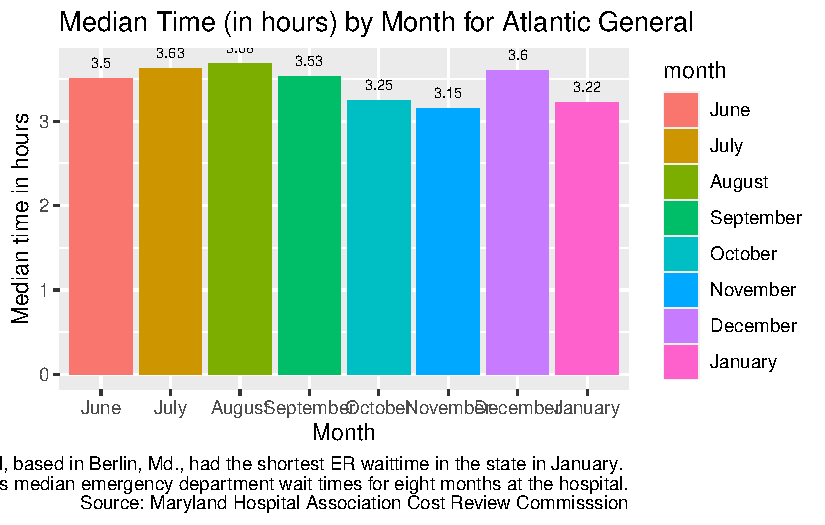
\includegraphics{Condon_MD_HOSPITAL_DATA_FINAL_files/figure-pdf/unnamed-chunk-6-1.pdf}

Findings from charts:

Atlantic General in Berlin, Md. had the highest median wait time in
January, and UM Eastern Shore in Easton, Md. had the longest median wait
time that month.

Atlantic General had a significantly shorter average wait time (of about
3.2 hours in its emergency department, which is still long) than UM
Eastern Shore at 29.5 hours. The variation in Eastern Shore's times was
also a significantly larger range. I was shocked to see that from
November to January, UM Eastern Shore's wait time increased by almost
1000 minutes on average.

From this data, I would want to talk to someone at each hospital to ask
what was going on. I'd also be interested in talking to people who
visited UM Eastern Shore and waited 1700 minutes (over 28 hours) to be
seen in an emergency room.

I also want to look into UM Eastern Shores' outlined objectives and
goals for decreasing times that are required to be stated under the new
EDDIE program. How does the hospital's objectives relate to the reality
of its extremely flunctuating wait times for patients.

Q2: What hospitals in Maryland are seeing the most and least improvement
in wait times? 1a. Which 5 hospitals had the lowest percent change since
base month? 1b. How many hospitals have had increasing wait times from
their base month to January? Which 5 have had the biggest increases?

\begin{Shaded}
\begin{Highlighting}[]
\NormalTok{Pct\_change }\OtherTok{\textless{}{-}}\NormalTok{ ED1a }\SpecialCharTok{\%\textgreater{}\%} 
  \FunctionTok{select}\NormalTok{(abbreviated\_name, august\_median, january\_median) }

\NormalTok{Pct\_change }\OtherTok{\textless{}{-}}\NormalTok{ Pct\_change }\SpecialCharTok{\%\textgreater{}\%}
  \FunctionTok{select}\NormalTok{(abbreviated\_name,august\_median, january\_median) }\SpecialCharTok{\%\textgreater{}\%} 
    \FunctionTok{mutate}\NormalTok{(}\AttributeTok{base\_august=}\NormalTok{ (january\_median }\SpecialCharTok{{-}}\NormalTok{ august\_median)}\SpecialCharTok{/}\NormalTok{august\_median }\SpecialCharTok{*}\DecValTok{100}\NormalTok{) }


\NormalTok{Pct\_change\_top5 }\OtherTok{\textless{}{-}}\NormalTok{ Pct\_change }\SpecialCharTok{\%\textgreater{}\%} 
  \FunctionTok{arrange}\NormalTok{(base\_august) }\SpecialCharTok{\%\textgreater{}\%} 
  \FunctionTok{head}\NormalTok{(}\DecValTok{5}\NormalTok{)}

\CommentTok{\#Answer: White Oak in Silver Spring, Md. (at {-}427.8\%), UMMC Midtwon in Baltimore (at {-}15.4), Mercy Hospital in Baltimore (at {-}14.4\%,), Atlantic General in Berlin, Md. (at {-}12.7\%) and Shady Grove in Rockville (at {-}10.5\%) had the lowest percent change, and thus the biggest decreases in hospital wait times since their base month.}
\end{Highlighting}
\end{Shaded}

How many hospitals have had increasing wait times from their base month
to January? Which 5 have had the biggest increases?

\begin{Shaded}
\begin{Highlighting}[]
\NormalTok{Pct\_change2 }\OtherTok{\textless{}{-}}\NormalTok{ ED1a }\SpecialCharTok{\%\textgreater{}\%} 
  \FunctionTok{select}\NormalTok{(abbreviated\_name, august\_median, january\_median) }

\CommentTok{\#Answer: 33 hospitals have increasing wait times since their base month.}

\NormalTok{Pct\_change2 }\OtherTok{\textless{}{-}}\NormalTok{ ED1a }\SpecialCharTok{\%\textgreater{}\%} 
  \FunctionTok{select}\NormalTok{(abbreviated\_name,august\_median, january\_median) }\SpecialCharTok{\%\textgreater{}\%} 
    \FunctionTok{mutate}\NormalTok{(}\AttributeTok{base\_august=}\NormalTok{ (january\_median }\SpecialCharTok{{-}}\NormalTok{ august\_median)}\SpecialCharTok{/}\NormalTok{august\_median }\SpecialCharTok{*}\DecValTok{100}\NormalTok{) }\SpecialCharTok{\%\textgreater{}\%} 
  \FunctionTok{arrange}\NormalTok{(}\FunctionTok{desc}\NormalTok{(base\_august)) }\SpecialCharTok{\%\textgreater{}\%} 
  \FunctionTok{head}\NormalTok{(}\DecValTok{5}\NormalTok{)}
  
\CommentTok{\#Answer: Of the 33 hospitals, the five with the highest increasing wait times were Upper Chesapeake in Bel Air, Md. (at 136.6\%), MedStar Good Samaritan in Baltimore (at 84.9\%), Carroll Hospital in Westminster, Md. (at 76.3\%), Union ChristianaCare in Elkton, Md. (at 62.6\%) and Holy Cross Germantown in Oakland, Md. (at 60.5\%).}
\end{Highlighting}
\end{Shaded}

Q3: How does Maryland's average ED wait time compare to the rest of the
country?

\begin{Shaded}
\begin{Highlighting}[]
\NormalTok{national\_ed }\OtherTok{\textless{}{-}}\NormalTok{ rio}\SpecialCharTok{::}\FunctionTok{import}\NormalTok{(}\StringTok{"Timely\_and\_Effective\_Care{-}State.csv"}\NormalTok{) }\SpecialCharTok{\%\textgreater{}\%} 
  \FunctionTok{clean\_names}\NormalTok{()}

\CommentTok{\#Data from Census for Medicare and Medicaid services: https://data.cms.gov/provider{-}data/dataset/apyc{-}v239 }

\NormalTok{national\_ed\_op18c }\OtherTok{\textless{}{-}}\NormalTok{ national\_ed }\SpecialCharTok{\%\textgreater{}\%} 
  \FunctionTok{filter}\NormalTok{(measure\_id }\SpecialCharTok{==} \StringTok{"OP\_18c"}\NormalTok{) }\SpecialCharTok{\%\textgreater{}\%} 
  \FunctionTok{mutate}\NormalTok{(}\AttributeTok{score =} \FunctionTok{gsub}\NormalTok{(}\StringTok{"[\^{}0{-}9.]"}\NormalTok{, }\StringTok{""}\NormalTok{, score)) }\SpecialCharTok{\%\textgreater{}\%}
  \FunctionTok{mutate}\NormalTok{(}\AttributeTok{score =} \FunctionTok{as.numeric}\NormalTok{(score))}

\CommentTok{\#I used OP\_18C because this is the outpatient category that aggregates psych and non{-}psych admits.}

\NormalTok{top10}\OtherTok{\textless{}{-}}\NormalTok{ national\_ed\_op18c }\SpecialCharTok{\%\textgreater{}\%} 
  \FunctionTok{arrange}\NormalTok{(}\FunctionTok{desc}\NormalTok{(score)) }\SpecialCharTok{\%\textgreater{}\%} 
  \FunctionTok{head}\NormalTok{(}\DecValTok{10}\NormalTok{)}
  
\FunctionTok{mean}\NormalTok{(national\_ed\_op18c}\SpecialCharTok{$}\NormalTok{score, }\AttributeTok{na.rm=}\ConstantTok{TRUE}\NormalTok{) }\CommentTok{\#= 267.3077}
\end{Highlighting}
\end{Shaded}

\begin{verbatim}
[1] 267.3077
\end{verbatim}

\begin{Shaded}
\begin{Highlighting}[]
\CommentTok{\#This data set, which collected wait times up until May 30, 2023, put Maryland at number 3 for the longest average emergency department times in the country. Maryland\textquotesingle{}s average wait time of 409 minutes, or almost 7 hours, was only shorter than DC and Vermont. The average of all of these median times was 267.3077 or 4.5 hours.}
\end{Highlighting}
\end{Shaded}

Map of 10 states with longest ED wait times

\begin{Shaded}
\begin{Highlighting}[]
\NormalTok{top10}\SpecialCharTok{$}\NormalTok{state }\OtherTok{\textless{}{-}} \FunctionTok{factor}\NormalTok{(top10}\SpecialCharTok{$}\NormalTok{state, }\AttributeTok{levels =}  \FunctionTok{c}\NormalTok{(}\StringTok{"DC"}\NormalTok{, }\StringTok{"VT"}\NormalTok{, }\StringTok{"MD"}\NormalTok{, }\StringTok{"DE"}\NormalTok{, }\StringTok{"RI"}\NormalTok{, }\StringTok{"MA"}\NormalTok{, }\StringTok{"PR"}\NormalTok{, }\StringTok{"TN"}\NormalTok{, }\StringTok{"NY"}\NormalTok{, }\StringTok{"GA"}\NormalTok{))}

\NormalTok{top10 }\SpecialCharTok{\%\textgreater{}\%} 
  \FunctionTok{ggplot}\NormalTok{(}\FunctionTok{aes}\NormalTok{(}\AttributeTok{x=}\NormalTok{state, }\AttributeTok{y=}\NormalTok{score, }\AttributeTok{weight=}\NormalTok{score, }\AttributeTok{fill=}\NormalTok{score)) }\SpecialCharTok{+}
   \FunctionTok{geom\_col}\NormalTok{()}\SpecialCharTok{+}
  \FunctionTok{geom\_text}\NormalTok{(}\FunctionTok{aes}\NormalTok{(}\AttributeTok{label=}\NormalTok{score), }\AttributeTok{vjust =} \SpecialCharTok{{-}}\DecValTok{1}\NormalTok{, }\AttributeTok{size =} \FloatTok{2.5}\NormalTok{) }\SpecialCharTok{+}
  \FunctionTok{labs}\NormalTok{(}
    \AttributeTok{title=}\StringTok{"States with longest Emergency Department Wait Time"}\NormalTok{,}
    \AttributeTok{x =} \StringTok{"State"}\NormalTok{,}
    \AttributeTok{y =} \StringTok{"Average (median) time in minutes patients spent in the emergency department before leaving from the visit"}\NormalTok{,}
    \AttributeTok{caption =} \StringTok{"source: Census for Medicare and Medicaid Services"}\NormalTok{)}
\end{Highlighting}
\end{Shaded}

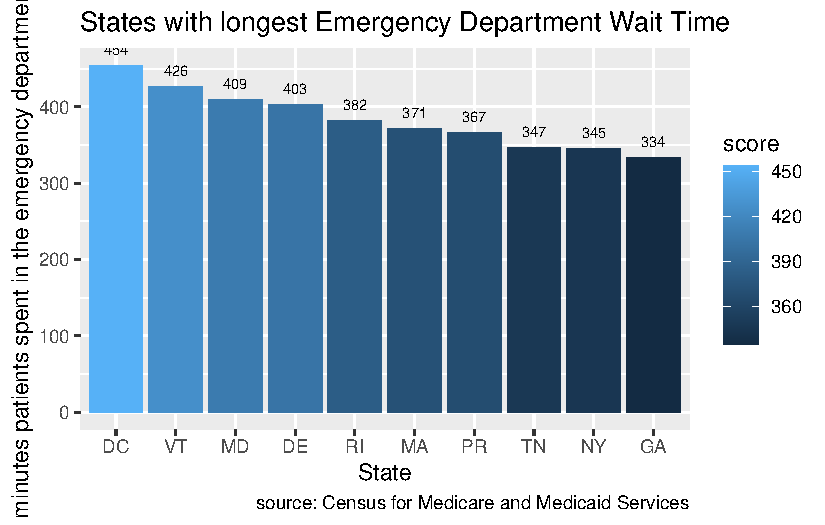
\includegraphics{Condon_MD_HOSPITAL_DATA_FINAL_files/figure-pdf/unnamed-chunk-10-1.pdf}

Q4: Are there any patterns between urban and rural hospitals? What
factors affect wait times in each of these areas?

\begin{Shaded}
\begin{Highlighting}[]
\CommentTok{\#Defining rural and urban (not rural) by MD Dept of Health definition}

\NormalTok{urban\_rural }\OtherTok{\textless{}{-}}\NormalTok{ january\_ed }\SpecialCharTok{\%\textgreater{}\%} 
  \FunctionTok{mutate}\NormalTok{(}\AttributeTok{county=}\NormalTok{city) }

\NormalTok{urban\_rural }\OtherTok{\textless{}{-}}\NormalTok{ urban\_rural }\SpecialCharTok{\%\textgreater{}\%}
   \FunctionTok{mutate}\NormalTok{(}\AttributeTok{county =} \FunctionTok{case\_when}\NormalTok{(}
\NormalTok{     county }\SpecialCharTok{==} \StringTok{"Berlin"} \SpecialCharTok{\textasciitilde{}} \StringTok{"Worcester"}\NormalTok{,}
\NormalTok{     county }\SpecialCharTok{==} \StringTok{"Oakland"} \SpecialCharTok{\textasciitilde{}} \StringTok{"Garrett"}\NormalTok{,}
\NormalTok{     county }\SpecialCharTok{==} \StringTok{"Baltimore"} \SpecialCharTok{\textasciitilde{}} \StringTok{"Balt City"}\NormalTok{,}
\NormalTok{     county }\SpecialCharTok{==} \StringTok{"Leonardtown"} \SpecialCharTok{\textasciitilde{}} \StringTok{"St. Marys"}\NormalTok{,}
\NormalTok{     county }\SpecialCharTok{==} \StringTok{"Hagerstown"} \SpecialCharTok{\textasciitilde{}} \StringTok{"Washington"}\NormalTok{,}
\NormalTok{     county }\SpecialCharTok{==} \StringTok{"Elkton"} \SpecialCharTok{\textasciitilde{}} \StringTok{"Cecil"}\NormalTok{,}
\NormalTok{    county }\SpecialCharTok{==} \StringTok{"Salisbury"} \SpecialCharTok{\textasciitilde{}} \StringTok{"Wicomico"}\NormalTok{,}
\NormalTok{     county }\SpecialCharTok{==} \StringTok{"Germantown"} \SpecialCharTok{\textasciitilde{}} \StringTok{"Montgomery"}\NormalTok{,}
\NormalTok{     county }\SpecialCharTok{==} \StringTok{"Havre De Grace"} \SpecialCharTok{\textasciitilde{}} \StringTok{"Harford"}\NormalTok{,}
\NormalTok{     county }\SpecialCharTok{==} \StringTok{"Rockville"} \SpecialCharTok{\textasciitilde{}} \StringTok{"Montgomery"}\NormalTok{,}
\NormalTok{     county }\SpecialCharTok{==} \StringTok{"Cumberland"} \SpecialCharTok{\textasciitilde{}} \StringTok{"Allegany"}\NormalTok{,}
\NormalTok{     county }\SpecialCharTok{==} \StringTok{"Silver Spring"} \SpecialCharTok{\textasciitilde{}} \StringTok{"Montgomery"}\NormalTok{,}
\NormalTok{     county }\SpecialCharTok{==} \StringTok{"Bethesda"} \SpecialCharTok{\textasciitilde{}} \StringTok{"Montgomery"}\NormalTok{,}
\NormalTok{     county }\SpecialCharTok{==} \StringTok{"La Plata"} \SpecialCharTok{\textasciitilde{}} \StringTok{"Charles"}\NormalTok{,}
\NormalTok{     county }\SpecialCharTok{==} \StringTok{"Fort Washington"} \SpecialCharTok{\textasciitilde{}} \StringTok{"Prince George\textquotesingle{}s"}\NormalTok{,}
\NormalTok{     county }\SpecialCharTok{==} \StringTok{"Olney"} \SpecialCharTok{\textasciitilde{}} \StringTok{"Montgomery"}\NormalTok{,}
\NormalTok{     county }\SpecialCharTok{==} \StringTok{"Glen Burnie"} \SpecialCharTok{\textasciitilde{}} \StringTok{"Anne Arundel"}\NormalTok{,}
\NormalTok{     county }\SpecialCharTok{==} \StringTok{"Columbia"} \SpecialCharTok{\textasciitilde{}} \StringTok{"Howard"}\NormalTok{,}
\NormalTok{     county }\SpecialCharTok{==} \StringTok{"Bel Air"} \SpecialCharTok{\textasciitilde{}} \StringTok{"Harford"}\NormalTok{,}
\NormalTok{     county }\SpecialCharTok{==} \StringTok{"Largo"} \SpecialCharTok{\textasciitilde{}} \StringTok{"Prince George\textquotesingle{}s"}\NormalTok{,}
\NormalTok{     county }\SpecialCharTok{==} \StringTok{"Easton"} \SpecialCharTok{\textasciitilde{}} \StringTok{"Talbot"}\NormalTok{,}
\NormalTok{     county }\SpecialCharTok{==} \StringTok{"Randallstown"} \SpecialCharTok{\textasciitilde{}} \StringTok{"Balt County"}\NormalTok{,}
\NormalTok{     county }\SpecialCharTok{==} \StringTok{"Annapolis"} \SpecialCharTok{\textasciitilde{}} \StringTok{"Anne Arundel"}\NormalTok{,}
\NormalTok{     county }\SpecialCharTok{==} \StringTok{"Clinton"} \SpecialCharTok{\textasciitilde{}} \StringTok{"Prince George\textquotesingle{}s"}\NormalTok{,}
\NormalTok{     county }\SpecialCharTok{==} \StringTok{"Towson"} \SpecialCharTok{\textasciitilde{}} \StringTok{"Balt County"}\NormalTok{,}
     \ConstantTok{TRUE} \SpecialCharTok{\textasciitilde{}}\NormalTok{ county  }
\NormalTok{   ))}
\end{Highlighting}
\end{Shaded}

According to MD Dept of health
(https://health.maryland.gov/pophealth/Pages/Rural-health.aspx):
``Allegany, Calvert, Caroline, Carroll, Cecil, Charles, Dorchester,
Frederick, Garrett, Harford, Kent, Queen Anne's, Somerset, St.~Mary's,
Talbot, Washington, Wicomico, and Worcester.''

\begin{Shaded}
\begin{Highlighting}[]
\NormalTok{urban\_rural }\OtherTok{\textless{}{-}} \FunctionTok{as.data.frame}\NormalTok{(urban\_rural)}

\NormalTok{urban\_rural }\OtherTok{\textless{}{-}} \FunctionTok{clean\_names}\NormalTok{(urban\_rural)}


\NormalTok{urban\_rural }\OtherTok{\textless{}{-}}\NormalTok{ urban\_rural }\SpecialCharTok{\%\textgreater{}\%} 
  \FunctionTok{mutate}\NormalTok{(}
  \AttributeTok{define =} \FunctionTok{case\_when}\NormalTok{(}
\NormalTok{   county }\SpecialCharTok{==} \StringTok{\textquotesingle{}Allegany\textquotesingle{}}  \SpecialCharTok{\textasciitilde{}} \StringTok{"rural"}\NormalTok{,}
\NormalTok{   county }\SpecialCharTok{==} \StringTok{\textquotesingle{}Cecil\textquotesingle{}} \SpecialCharTok{\textasciitilde{}} \StringTok{"rural"}\NormalTok{,}
\NormalTok{   county }\SpecialCharTok{==} \StringTok{\textquotesingle{}Charles\textquotesingle{}}  \SpecialCharTok{\textasciitilde{}} \StringTok{"rural"}\NormalTok{,}
\NormalTok{   county }\SpecialCharTok{==} \StringTok{\textquotesingle{}Federick\textquotesingle{}}  \SpecialCharTok{\textasciitilde{}} \StringTok{"rural"}\NormalTok{,}
\NormalTok{   county }\SpecialCharTok{==} \StringTok{\textquotesingle{}Garrett\textquotesingle{}} \SpecialCharTok{\textasciitilde{}} \StringTok{"rural"}\NormalTok{,}
\NormalTok{   county }\SpecialCharTok{==} \StringTok{\textquotesingle{}Harford\textquotesingle{}}  \SpecialCharTok{\textasciitilde{}} \StringTok{"rural"}\NormalTok{,}
\NormalTok{   county }\SpecialCharTok{==} \StringTok{\textquotesingle{}St. Marys\textquotesingle{}}  \SpecialCharTok{\textasciitilde{}} \StringTok{"rural"}\NormalTok{,}
\NormalTok{   county }\SpecialCharTok{==} \StringTok{\textquotesingle{}Talbot\textquotesingle{}} \SpecialCharTok{\textasciitilde{}} \StringTok{"rural"}\NormalTok{,}
\NormalTok{   county }\SpecialCharTok{==} \StringTok{\textquotesingle{}Washington\textquotesingle{}}  \SpecialCharTok{\textasciitilde{}} \StringTok{"rural"}\NormalTok{,}
\NormalTok{   county }\SpecialCharTok{==} \StringTok{\textquotesingle{}Wicomico\textquotesingle{}} \SpecialCharTok{\textasciitilde{}} \StringTok{"rural"}\NormalTok{,}
\NormalTok{   county }\SpecialCharTok{==} \StringTok{\textquotesingle{}Worcester\textquotesingle{}}  \SpecialCharTok{\textasciitilde{}} \StringTok{"rural"}\NormalTok{,}
   \ConstantTok{TRUE} \SpecialCharTok{\textasciitilde{}} \StringTok{"not\_rural"}\NormalTok{))}

\NormalTok{urban\_rural }\OtherTok{\textless{}{-}}\NormalTok{ urban\_rural }\SpecialCharTok{\%\textgreater{}\%} 
  \FunctionTok{select}\NormalTok{(abbreviated\_name, january\_median, address, county, define)}
\end{Highlighting}
\end{Shaded}

\begin{Shaded}
\begin{Highlighting}[]
\NormalTok{rural\_hospitals }\OtherTok{\textless{}{-}}\NormalTok{ urban\_rural }\SpecialCharTok{\%\textgreater{}\%} 
  \FunctionTok{filter}\NormalTok{(define }\SpecialCharTok{==} \StringTok{"rural"}\NormalTok{)}

\FunctionTok{mean}\NormalTok{(rural\_hospitals}\SpecialCharTok{$}\NormalTok{january\_median) }\CommentTok{\#= 682.25 minutes (or 11.3 hours)}
\end{Highlighting}
\end{Shaded}

\begin{verbatim}
[1] 698.1538
\end{verbatim}

\begin{Shaded}
\begin{Highlighting}[]
\NormalTok{not\_rural\_hospitals }\OtherTok{\textless{}{-}}\NormalTok{ urban\_rural }\SpecialCharTok{\%\textgreater{}\%} 
  \FunctionTok{filter}\NormalTok{(define }\SpecialCharTok{==} \StringTok{"not\_rural"}\NormalTok{)}

\FunctionTok{mean}\NormalTok{(not\_rural\_hospitals}\SpecialCharTok{$}\NormalTok{january\_median) }\CommentTok{\#= 711.2759 minutes (or 11.8 hours)}
\end{Highlighting}
\end{Shaded}

\begin{verbatim}
[1] 704.9286
\end{verbatim}

\begin{Shaded}
\begin{Highlighting}[]
\CommentTok{\#There is not a significant difference in averages for January wait times for rural and non rural hospitals}
\end{Highlighting}
\end{Shaded}

\begin{Shaded}
\begin{Highlighting}[]
\NormalTok{urban\_rural }\OtherTok{\textless{}{-}}\NormalTok{ urban\_rural }\SpecialCharTok{\%\textgreater{}\%}
  \FunctionTok{mutate}\NormalTok{(}\AttributeTok{name2 =} \FunctionTok{substr}\NormalTok{(}\FunctionTok{str\_replace\_all}\NormalTok{(}\FunctionTok{tolower}\NormalTok{(abbreviated\_name), }\StringTok{"[\^{}[:alnum:]]"}\NormalTok{, }\StringTok{""}\NormalTok{), }\DecValTok{1}\NormalTok{, }\DecValTok{10}\NormalTok{))}

\NormalTok{urban\_rural }\SpecialCharTok{\%\textgreater{}\%} 
  \FunctionTok{ggplot}\NormalTok{(}\FunctionTok{aes}\NormalTok{(}\AttributeTok{x=}\FunctionTok{reorder}\NormalTok{(name2, january\_median), }\AttributeTok{y=}\NormalTok{january\_median, }\AttributeTok{weight=}\NormalTok{january\_median, }\AttributeTok{fill=}\NormalTok{define)) }\SpecialCharTok{+}
  \FunctionTok{geom\_col}\NormalTok{()}\SpecialCharTok{+}
  \FunctionTok{geom\_text}\NormalTok{(}\FunctionTok{aes}\NormalTok{(}\AttributeTok{label=}\NormalTok{january\_median), }\AttributeTok{vjust =} \SpecialCharTok{{-}}\DecValTok{1}\NormalTok{, }\AttributeTok{size =} \DecValTok{2}\NormalTok{, }\AttributeTok{angle =} \DecValTok{90}\NormalTok{) }\SpecialCharTok{+}
  \FunctionTok{theme}\NormalTok{(}\AttributeTok{axis.text.x =} \FunctionTok{element\_text}\NormalTok{(}\AttributeTok{angle =} \DecValTok{90}\NormalTok{)) }\SpecialCharTok{+}
  \FunctionTok{labs}\NormalTok{(}
    \AttributeTok{title=}\StringTok{"Median Time for hospitals in January (by rural and non"}\NormalTok{,}
    \AttributeTok{x =} \StringTok{"Hospital Name"}\NormalTok{,}
    \AttributeTok{y =} \StringTok{"median time in minutes"}\NormalTok{,}
    \AttributeTok{caption =} \StringTok{"source: Maryland Hospital Association Cost Review Commisssion"}\NormalTok{)}
\end{Highlighting}
\end{Shaded}

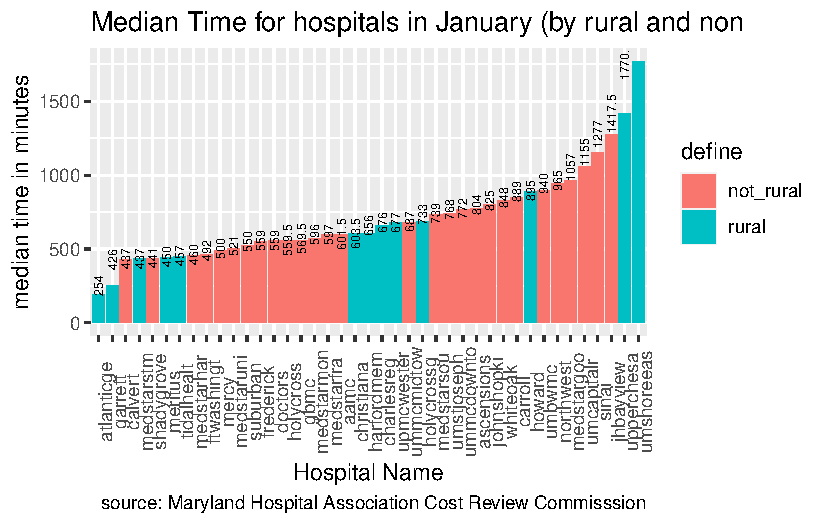
\includegraphics{Condon_MD_HOSPITAL_DATA_FINAL_files/figure-pdf/unnamed-chunk-14-1.pdf}

\begin{Shaded}
\begin{Highlighting}[]
\CommentTok{\#Although the two hospitals with the highest average wait times in January were rural, the hospitals with the two lowest wait times were also rural. There seems to be no causal relationship between wait times and rural or urban hospitals.}
\end{Highlighting}
\end{Shaded}

Q5: What hospital has seen the most improvement in its hospital wait
times?

\begin{Shaded}
\begin{Highlighting}[]
\CommentTok{\#Compared from August to January with each month\textquotesingle{}s difference to account for seasonal variations}

\NormalTok{ED1a }\OtherTok{\textless{}{-}}\NormalTok{ ED1a }\SpecialCharTok{\%\textgreater{}\%} 
  \FunctionTok{mutate}\NormalTok{(}\AttributeTok{change =}\NormalTok{ (august\_median }\SpecialCharTok{{-}}\NormalTok{ july\_median) }\SpecialCharTok{+}\NormalTok{ (september\_median }\SpecialCharTok{{-}}\NormalTok{ august\_median) }\SpecialCharTok{+}\NormalTok{ (october\_median }\SpecialCharTok{{-}}\NormalTok{ september\_median) }\SpecialCharTok{+}\NormalTok{ (november\_median }\SpecialCharTok{{-}}\NormalTok{ october\_median) }\SpecialCharTok{+}\NormalTok{ (december\_median }\SpecialCharTok{{-}}\NormalTok{ november\_median) }\SpecialCharTok{+}\NormalTok{ (january\_median }\SpecialCharTok{{-}}\NormalTok{ december\_median))}

\NormalTok{ED1a }\SpecialCharTok{\%\textgreater{}\%} 
  \FunctionTok{arrange}\NormalTok{(change) }\SpecialCharTok{\%\textgreater{}\%} 
  \FunctionTok{head}\NormalTok{(}\DecValTok{5}\NormalTok{)}
\end{Highlighting}
\end{Shaded}

\begin{verbatim}
  hospital_id abbreviated_name june_median rolling_median_june_ytd july_median
1      210038     UMMC MIDTOWN         685                   705.0         849
2      210034   MedStar Harbor         458                   529.5         553
3      210008            Mercy         526                   575.0         577
4      210016        White Oak        1251                  1283.0         865
5      210061 Atlantic General         210                   206.0         218
  rolling_median_july_ytd august_median rolling_median_august_ytd
1                     705           800                       723
2                     533           474                       532
3                     575           575                       569
4                    1203          1143                      1196
5                     200           221                       205
  september_median rolling_median_september_ytd october_median
1            658.5                          722            768
2            910.0                          977            513
3            407.0                          504            450
4            855.0                         1125           1328
5            212.0                          206            195
  rolling_median_october_ytd november_median rolling_median_november_ytd
1                        732             560                         713
2                        532             402                         511
3                        497             423                         489
4                       1114            1210                        1115
5                        203             189                         202
  december_median rolling_median_december_ytd january_median
1           698.0                       710.0            677
2           441.5                       482.5            457
3           466.0                       486.0            492
4           794.0                       786.0            825
5           216.0                       204.0            193
  rolling_median_january_ytd average_median_attainment
1                      698.0                  711.9375
2                      467.5                  526.0625
3                      482.0                  489.5000
4                      739.0                 1033.8750
5                      203.0                  206.7500
  change_from_base_month_to_latest_improvement x21 change
1                                           -8   0   -172
2                                           -1   0    -96
3                                          -34   0    -85
4                                         -426   0    -40
5                                          -17   0    -25
\end{verbatim}

\begin{Shaded}
\begin{Highlighting}[]
\CommentTok{\#UMMC Midtown in Baltimore saw the biggest improvement, dropping an aggregated 172 minutes from August through January. UM Eastern Shore in Easton added 819.5 minutes from August through January.}
\end{Highlighting}
\end{Shaded}

Conclusion:

\begin{enumerate}
\def\labelenumi{\arabic{enumi}.}
\tightlist
\item
  What are the average wait times for each hospital across the state in
  January in hours? As of January, what is month over month wait time
  for the hospitals with the longst and shortest wait times?
\end{enumerate}

Please see each hospital in January on this Data Wrapper: Map from data
wrapper: https://app.datawrapper.de/map/BTfas/publish In January,
University of Maryland Shore Eastern in Easton, Md. (Talbot County) had
the longest wait time at 1770.5 minutes, or 29.5 hours. See line 203 for
the graph of each month from June through August. \#In January, Atlantic
General, located in Berlin, Md (Worcester County) had the shortest wait
time at 193 minutes, or about 3.2 hours. See line 242 for the graph of
each month from June through August.

\begin{enumerate}
\def\labelenumi{\arabic{enumi}.}
\setcounter{enumi}{1}
\tightlist
\item
  What hospitals in Maryland are seeing the most and least improvement
  in wait times? 1a. Which 5 hospitals had the biggest improvement in
  wait times measured by the lowest percent change since base month?
\end{enumerate}

White Oak in Silver Spring, Md. (at -427.8\%), UMMC Midtwon in Baltimore
(at -15.4\%), Mercy Hospital in Baltimore (at -14.4\%,), Atlantic
General in Berlin, Md. (at -12.7\%) and Shady Grove in Rockville (at
-10.5\%) had the lowest percent change, and thus the biggest decreases
in hospital wait times since their base month.

2b. How many hospitals have had increasing wait times from their base
month to January? Which 5 have had the biggest increases?

Answer: Of the 33 hospitals, the five with the highest increasing wait
times were Upper Chesapeake in Bel Air, Md. (at 136.6\%), MedStar Good
Samaritan in Baltimore (at 84.9\%), Carroll Hospital in Westminster, Md.
(at 76.3\%), Union ChristianaCare in Elkton, Md. (at 62.6\%) and Holy
Cross Germantown in Oakland, Md. (at 60.5\%).

\begin{enumerate}
\def\labelenumi{\arabic{enumi}.}
\setcounter{enumi}{2}
\tightlist
\item
  How does Maryland's average ED wait time compare to the rest of the
  country?
\end{enumerate}

The data from Census for Medicare and Medicaid services, which collected
wait times up until May 30, 2023, put Maryland at number 3 for the
longest average emergency department times in the country. Maryland's
average wait time of 409 minutes, or almost 7 hours, was only shorter
than DC and Vermont.

\begin{enumerate}
\def\labelenumi{\arabic{enumi}.}
\setcounter{enumi}{3}
\tightlist
\item
  Are there any patterns between urban and rural hospitals? What factors
  affect wait times in each of these areas?
\end{enumerate}

There is not a significant difference in averages for january wait times
for rural and non rural hospitals. (Please see graph on 362) Although
the two hospitals with the highest average wait times in January were
rural, the hospitals with the two lowest wait times were also rural.
There seems to be no causal relationship between wait times and rural or
urban hospitals.

\begin{enumerate}
\def\labelenumi{\arabic{enumi}.}
\setcounter{enumi}{4}
\tightlist
\item
  What hospital has seen the most improvement (and least) in its
  hospital wait times?
\end{enumerate}

UMMC Midtown in Baltimore saw the biggest improvement, dropped 172
minutes from August through January. UM Eastern Shore in Easton added
819.5 minutes from August through January.

250-word summary of the most interesting newsworthy findings so far: I
think the biggest takeaway from all of this is that the high hospital
wait times is a state-wide problem. There doesn't seem to be one
hospital as an outlier for the high wait times. Even Atlantic General in
Worcester County that had the shortest wait time at 3.2 hours in January
still had a very long wait time. In 2023, according to the Medicard
data, the US average median wait time was 267 minutes, or 4.45 hours. In
January in Maryland, only Atlantic and Garret fell below this number. So
39 out of 41 Maryland hospitals had a median time above the average
national median wait time. The hospitals with the most and least
improvements in wait times as a percentage also saw no type of pattern,
as they were all pretty scattered across the state.

There also was not even a pattern between the rural and urban hospitals.
This indicates that there is an issue in how the Maryland hospital
system as a whole responds to emergency care, as one cannot blame high
volumes of people or other factors which may be attributed to
demographic factors like neighborhood type.

UM Eastern Shore is a standout problem as having the highest wait time
in January and also having the largest change from August through
January in minutes.

All of this indicates to me that the data points to a clear issue in
hospitals that is present across the state, not just in one area or just
in rural or non-rural hospitals.

On-the-ground reporting would have to be done in order to really find
out what is going on with Maryland hospitals and to figure out what is
broken in the system.

Story Memo/Pitch:

Headline: Maryland hospital wait times see little improvement, despite
new state commission Author: Emily R. Condon Pitch: In June, the
Maryland Hospitals Association established EDDIE, the Emergency
Department Dramatic Improvements Effort, to address hospital wait times
in the state. By having each hospital set objectives for lowering
emergency department wait times and discharges, EDDIE aims to put
Maryland hospitals back on target with the rest of the country. This
analysis of data from EDDIE shows that hospital wait times in the state
are still suffering. There doesn't seem to be one hospital as an outlier
for the high wait times. Even Atlantic General in Worcester County that
had the shortest wait time at 3.2 hours in January still had a very long
wait time. In 2023, according to the Medicard data, the US average
median wait time was 267 minutes, or 4.45 hours. In January in Maryland,
only Atlantic and Garret fell below this number. So 39 out of 41
Maryland hospitals had a median time above the average national median
wait time. The hospitals with the most and least improvements in wait
times as a percentage also saw no type of pattern, as they were all
pretty scattered across the state. While reporting has been done on
this, solutions-oriented articles lack. I would do on-the-ground
reporting and find hospitals who are seeing some improvements to talk to
them about what they are doing to improve emergency department
waittimes. Estimated Word Count: 800 words Potential photos / videos:
Photos of people in Emergency Rooms are difficult due to HIPPA laws, so
outside shots of hospitals Potential graphics: Graphs of each hospital,
MD median wait time compares to other states, a statewide map with each
hospital and their most recent media wait time



\end{document}
